\documentclass[11pt,a4paper]{report}
\usepackage{graphicx,color}
\usepackage[english]{babel}
\usepackage[T1]{fontenc}
\usepackage{iftex}
\usepackage{color}
\usepackage{listings}
\usepackage{amsmath}
\usepackage{mathtools}
\ifPDFTeX
    \usepackage[utf8]{inputenc}
\fi

\IfFileExists{tuereport2008.sty}{\usepackage[english]{tuereport2008}}{}

\lstset{language=[Sharp]C, breaklines=true}

\IfFileExists{tuereport2008.sty}
{
    \title{Simulation in computer graphics}
    \subtitle{Project 2}
    \author{Michiel Fortuin\\Wouter Boereboom}
    \version{1.0}
    \administrativeunit{Department of Mathematics and Computer Science}   % insert department name here
    \department{Visualization}     % subdepartment, or group
}{
    \title{Simulation in computer graphics: project 1}
    \author{Michiel Fortuin\\Wouter Boereboom}
}
%\orderissuer{}
%\copyholder{}
%\website{}
%\reference{}

\begin{document}
\maketitle

\tableofcontents

\chapter{Introduction}

This report covers a description of the implementation of fluid simulation techniques. It deals with basic fluid techniques, boundaries, rigid bodies and fluid coupling. A few scenes are used to show things that can be created using these techniques. The scope of this report will consist out of a basic explanation of the implemented techniques, as well as a technical description of how these techniques were implemented. This will be done using formulas, images and descriptions of interesting technical aspects. The application described in this document is developed in $C\#$ and is tested and debugged under windows 7. 
\chapter{Overview}

\chapter{Interaction}
There are several types of user interaction within the simulation which can be put in two categories; interaction that directly influences the simulation (adds forces) and interaction that influences the simulation settings (change timestep, scene, etc.). \\

\smallskip
The intereaction that directly influences the simulation itself is the mouse interaction. When clicking and dragging on a particle (or its proximity) a spring force will be applied between the current mouse position and the particle. This makes it possible for the user to grab and drag particles around in the simulation. The mouse position is updated in every time step. \\

\smallskip
The keyboard commands that influence the settings of the simulation as well as the scenes are as follows: \\
\begin{itemize}
  \item \textbf{C}: Resets the current scene.
  \item \textbf{D}: Starts/Stops capturing frames.
  \item \textbf{Q}: Exit application.
  \item \textbf{space}: Pause simulation.
  \item \textbf{Up}: Doubles timestep $(dt=dt*2)$.
  \item \textbf{Down}: Halves timestep $(dt = dt/2)$.
  \item \textbf{Left}: halves number of steps skipped. \\ 
  (increases simulation computational effort) 
  \item \textbf{Right}: doubles number of steps skipped. \\
  (decreases computational effort)
  \item \textbf{1}: Switch to Euler solver.
  \item \textbf{2}: Switch to Mid-point solver.
  \item \textbf{3}: Switch to Runge-Kutta solver.
  \item \textbf{4}: Switch to Verlet solver.
  \item \textbf{f1}: Switch to simple particle scene.
  \item \textbf{f2}: Switch to cloth scene.
  \item \textbf{f3}: Switch to hair scene.
  \item \textbf{f4}: Switch to solar system scene.
\end{itemize}



\chapter{Basic fluid simulation}

In order to implement the more advanced fluid simulation techniques, a proper basic fluid simulation is an essential starting point. For this project an Eulerian fluid method has been used, based on the techniques described in "Real-Time Fluid Dynamics For Games" by Jos Stam. 

The techniques and tricks described in this paper are directly ported into the fluid simulation application used in this project. This is the case for basic physics, the grid structure used to calculate both the density and velocity fields as well as the basic solving routine for fluid simulations. The part describing the boundaries has been implemented and extended to work for the physical simulation bounding box as well as for fixed objects within the simulation. 

The basic fluid simulation is also extended with mouse interaction. by clicking and dragging the mouse, a force can be added to the simulation.  
\chapter{Boundaries and Fixed objects}

As described before, the base Boundary implementation has been based on the paper "Real-Time Fluid Dynamics for Games" by Jos Stam. This method consists out of the treatment of all boundary cells around the simulation and altering these such that fluids will bounce of these "wall"-cells rather than flow through them. 

To adapt this technique to work for fixed objects within the simulation, a classification is done for every cell. For each cell there are four categories;"Empty", "Invert", "Copy" and "Zero". "Empty" is a classification for a cell that is not part of any sort of object or border. Fluids can flow through this cell normally. "Invert"means an incoming force or density has to be inverted back from where it came originally. This classification needs a source as well, in order to know what cell the force has to be directed at. "Copy" copies the velocity or density from a neighbouring cell from a set source. "Zero" cells are cells through which no fluids can flow at all, like the inside of solid objects. The source of the "invert" and "copy" cells is based on the positioning of this cell on the solid object the fluid needs to flow around. 

This boundary classification together with their associated source is made and saved in a list for the velocities in horizontal direction and vertical direction as well as the density field. These are done seperately, as different boundary conditions and classifications apply to forces coming from different directions (again as described by Stam). 


\chapter{Rigid Bodies}
Rigid body's are defined by a particle that is the center of mass and a polygon. The weight distribution is equal in the complete rigid body.

To find points where forces has to be applied, a discrete version of the rigid body has to be found. This is simple done by walking over the bounding box and checking if the cell at that position is in the polygon. Let $P$ the position that is checked.

It is also interesting to know to which points it is connected. This is done by checking the horizontal neighbours and vertical neighbours. Let this be $A_{P,1} .. A_{P,4}$. With this information all the boundary cells can be detected of a rigid object.

\section{User interaction}
It is possible to interact with the rigid object. If a rigid object is selected with the mouse, a spring force is created between the mouse and the particle at the center of the object.

\section{Boundaries}
With the information found it is easy to create boundaries for the liquid. For every adjacent cell the correct classification is determined. These classifications are described in chapter \ref{chap:BoundariesAndFixedObjects}.

\section{Body's to fluid}
Forces that are exerted on $A_{P,1} .. A_{P,4}$ (if they are liquid) is based on the velocity of cell $P$ in the object. The velocity  and the angular velocity of the object are both used to calculate the velocity of point $P$. This velocity is multiplied with a constant, before applying it to the fluid. In figure \ref{fig:BodyToFluid} there is a scene where forces are applied from the body to the fluid.

\begin{figure}[htb!]
    \centering
    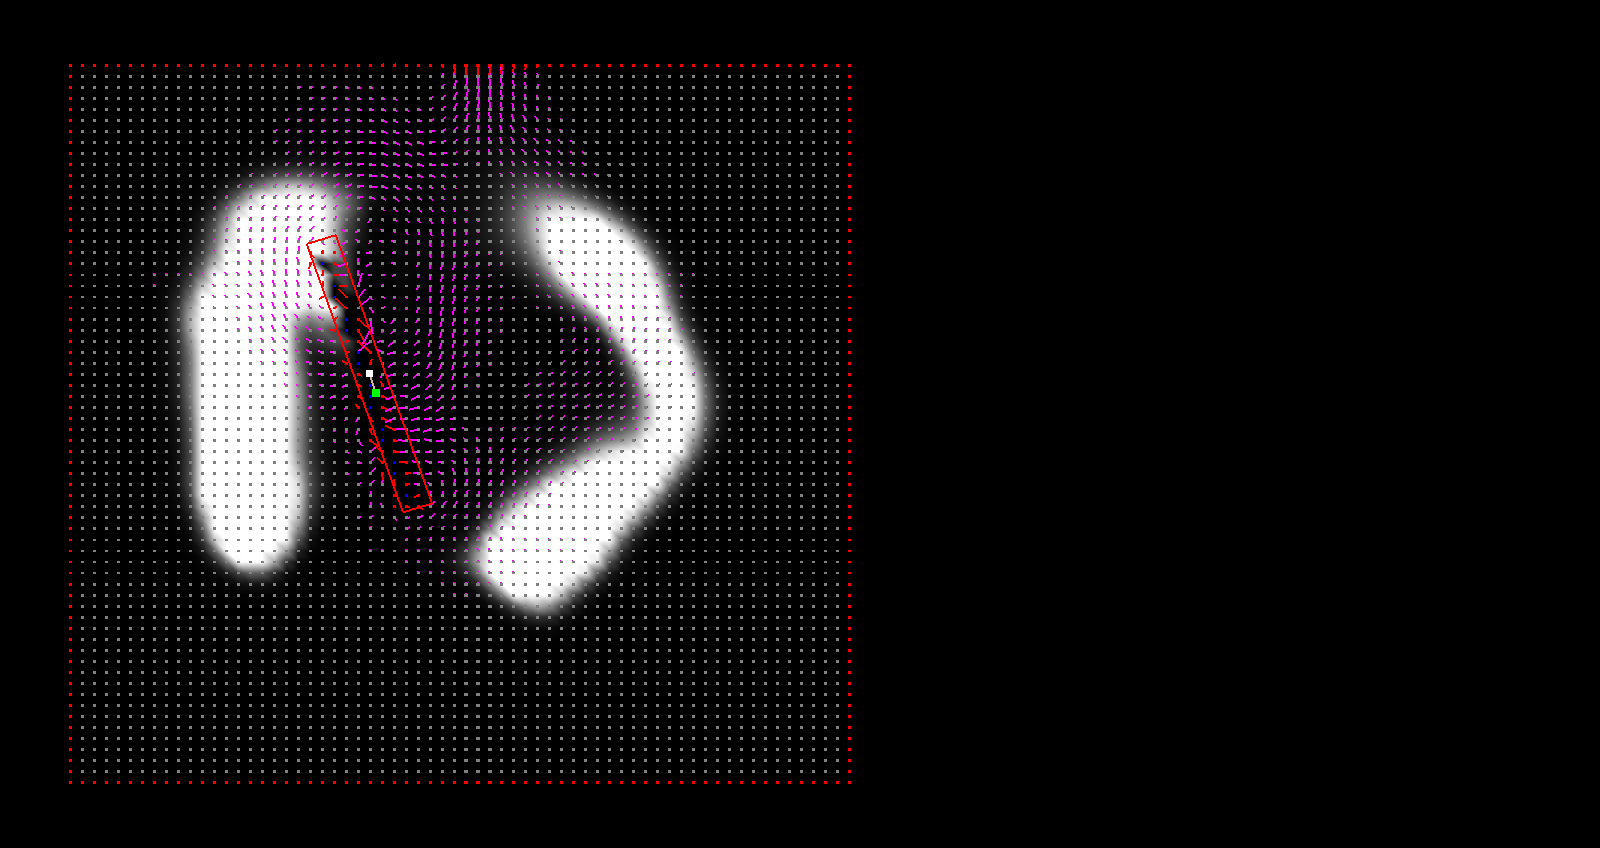
\includegraphics[width=0.6\textwidth]{images/BodyToFluid}
    \caption{A scene where forces from the body are applied to the fluid}
    \label{fig:BodyToFluid}
\end{figure}

\section{Fluid to Body's}
The force on point $P$ is calculated by the velocity in the adjacent cells $A_{P,1} .. A_{P,4}$ if there is liquid. The velocity is multiplied with it's density at that point and a constant. The force on point $P$ is then transformed to linear force and rotation force on the object. In figure \ref{fig:FluidToBody} there is a scene where forces are applied from the fluid to the body. To create a more natural way of interacting with the rigid body a viscous drag is added, so it will stop when no force is being added.

\begin{figure}[htb!]
    \centering
    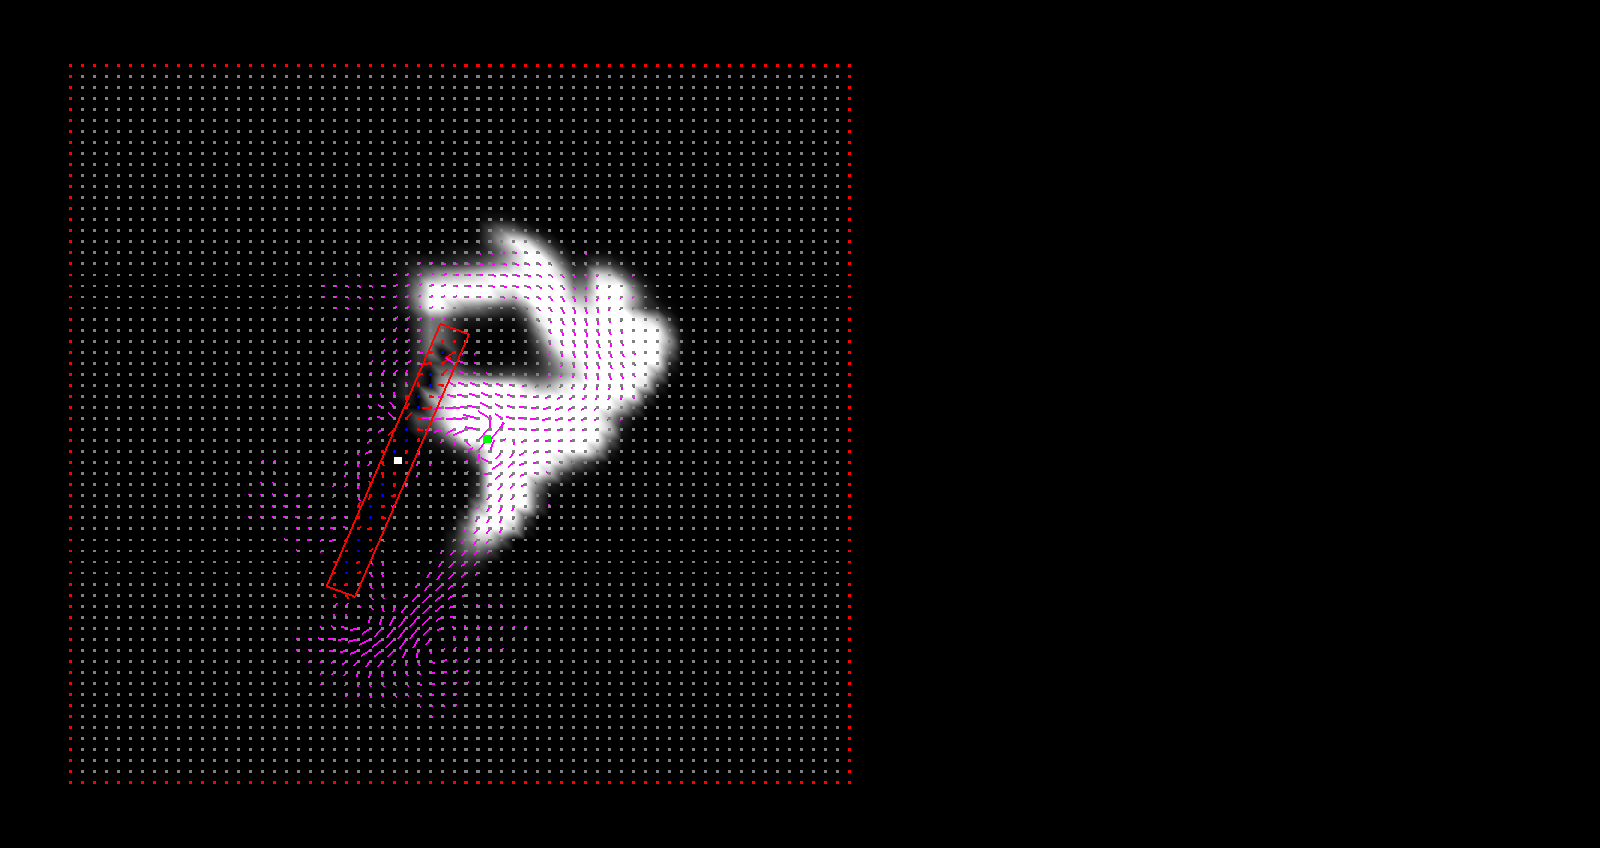
\includegraphics[width=0.6\textwidth]{images/FluidToBody}
    \caption{A scene where forces from the fluid are applied to the body}
    \label{fig:FluidToBody}
\end{figure}
\chapter{Particles}
\chapter{Conclusions}
The results are all in form of an application from which all the shown. Apart from some slight boundary issues, the application works well. All desired features and fluid behaviour works as described in this document. 
This application is well suited for future expansion. Techniques currently implemented can be perfected, and there are several other fluid simulation techniques that can be implemented to further improve the simulation.

\end{document}